%%%%%%%%%%%%%%%%%%%%%%%%%%%%%%%%%%% CABECALHO %%%%%%%%%%%%%%%%%%%%%%%%%%%%%%%%%%%
\documentclass[a4paper]{abnt}

\usepackage[utf8]{inputenc}
\usepackage{csquotes}
\usepackage[brazil]{babel}
\usepackage[T1]{fontenc}
\usepackage[all,defaultlines=2]{nowidow}
\usepackage[multiple]{footmisc}
\usepackage{xcolor,graphicx}
\usepackage[backend=bibtex,backref=true]{biblatex}
\usepackage[colorlinks=true,urlcolor=blue,linkcolor=black,citecolor=red]{hyperref}

\bibliography{projeto}

\author{Igor~Santos}
\title{Projeto~de~TCC - Insert~Coin}

\makeindex
\begin{document}
\maketitle

%%%%%%%%%%%%%%%%%%%%%%%%%%%%%%%%%%%%% INICIO %%%%%%%%%%%%%%%%%%%%%%%%%%%%%%%%%%%%%

\tableofcontents

\chapter{Proposta do Projeto de TCC}

O projeto a ser desenvolvido é um Sistema Pessoal de Planejamento Financeiro, ou de Controle Orçamentário, ou ainda, um Administrador de
Finanças. Seu objetivo é transformar a organização financeira de uma pessoa ou de uma residência, facilitando o manuseio e controle de entrada e saída do dinheiro e das contas bancárias, bem como do cartão de crédito – neste, alterando a forma como o usuário comumente vê o ``plástico''.

Em verdade, o principal diferencial do produto em relação à concorrência atual no mercado será o controle de cartões de crédito. O brasileiro tem o costume de considerar o cartão como um ``gasto'', uma despesa que atrapalha o bom andamento do orçamento familiar, sendo assim um ``mal necessário'' devido aos seus benefícios no adiamento de compras.

O objetivo do \textbf{Insert Coin} nesse sentido é auxiliar o usuário no entendimento dos seus cartões de crédito, e integrá-los ao seu fluxo de caixa normal. Tal fluxo é comumente baseado na entrada de poucas fontes de renda (de alto volume), e a saída em diversas despesas mensais (de volume menor). O cartão de crédito, por ser um concentrador de despesas que adia o pagamento de diversos eventos para um único dia, tende mais confundir do que a ajudar. O usuário precisa compreender bem a dinâmica dos dias de fechamento e de abertura de nova fatura, do ``melhor dia para compra'', o dia do vencimento e quais são os valores possíveis de pagamento – e quais as consequências de não pagar a fatura por completo. Além disso, o lançamento de despesas ocorre com diversos dias de diferença entre o evento e seu aparecimento na fatura parcial. Tudo isso vai muito além do fluxo simples de sua conta-corrente e seu cartão de débito, que consiste em receber o salário do mês, e lançamentos instantâneos do uso do cartão de débito.

%%%%%%%%%%%%%%%%%%%%%%%%%%%%%%%%%%%%%%%%%%%%%%%%%%%%%%%%%%%%%%%%%%%%%%%%%%%%%%%%%%%%%%%%%
\section{O Projeto}

Inicialmente chamado de \textbf{Insert Coin}, ele é principalmente um sistema baseado no lançamento de entradas e saídas de uma ou mais contas de finanças. Ele se assemelha à organização de um Livro-Caixa empresarial, onde o usuário marcará todos os valores recebidos e gastos de uma determinada conta. 

Atualmente existem diversos sistemas no mercado, tanto web quanto móvel, que atendem a esse tipo de usuário, auxiliando na visualização e controle das despesas mensais. Boa parte deles tem o mesmo princípio, inclusive. Portanto, se considerarmos somente esta \emph{feature}, o sistema será pouco diferente do que já existe no mercado e, por exemplo, não incentivará a migração dos usuários de concorrentes para o nosso projeto. Para remediar isso tentaremos inovar na interface e na facilidade de entrada de dados, que é um dos grandes obstáculos para a introdução deste tipo de sistema na rotina do usuário.

Por outro lado, somente um dos sistemas encontrados tenta suprir as peculiaridades do mercado de cartões de crédito nacional, de forma muito vaga e primariamente informativa. O método a ser utilizado aqui é bem mais ativo: ele auxilia o usuário a entender como o cartão de crédito afeta seu fluxo de caixa e insere, como despesas comuns, os eventos nos quais o cartão foi utilizado. O objetivo é evitar a segregação comum que o brasileiro faz em considerar o cartão de crédito com uma mais uma conta/boleto a pagar, como é a eletricidade ou a água da casa. No cartão são feitos gastos assim como ocorrem na conta de débito: lazer, vestuário, transporte, educação, etc. Portanto, porque devemos pensar em ``reduzir os gastos do cartão'' ao invés de ``reduzir os gastos mensais''?

Trabalhando de forma unificada será mais fácil para o usuário compreender o destino do dinheiro daquele mês. Também será possível começar a planejar e organizar metas de redução dos gastos, ou objetivos de economia de forma eficiente e focada. Essa unificação ocorrerá a partir da visualização das despesas daquele mês com relação às entradas; o usuário não precisará se perder em filtros de datas distintos entre a conta-corrente e o cartão de crédito -- que naturalmente possuem fluxos temporais diferenciados. O sistema também evitará a dúvida comum ``será que já posso usar o cartão de crédito?'', auxiliando o usuário a entender as datas importantes de seus cartões, e as inserindo na rotina que ele já conhece e compreende -- a de sua conta corrente e salário.

O que mais cria dúvidas no cartão de crédito é que sua fatura é finalizada cerca de 10 dias antes do dia de pagamento. Aquele período é quando o usuário não está certo de onde as despesas se encaixam melhor: se no mês atual ou no seguinte. Essa confusão se acentua pois as datas da fatura dificilmente encapsulam o período de mês com o qual o usuário está financeiramente acostumado: seu fluxo mensal de entrada do salário. Se ele decide colocar o vencimento do cartão para uma data próxima de seu salário, o fechamento da fatura fica distante do final do mês; se decide fechar a fatura no final do mês, o pagamento fica distante das outras contas que ele comumente paga. E muitas vezes algumas despesas de uma determinada só serão pagas dali a dois meses, o que gera confusão e certa negligência na hora de conferir a origem dos gastos.

A proposta é coletar as datas importantes do cartão e orientar o usuário para que, sempre que possível, a fatura seja paga em cheio no dia do vencimento (em débito automático, por exemplo). Esta é, de acordo com os especialistas da área, a melhor forma de conviver com o cartão, pois não gera juros adicionais em cima do que não foi pago. A partir daí, o usuário terá configurada sua conta-corrente do sistema para que as despesas que ocorrerem no cartão de crédito sejam visualizadas simultaneamente às da conta, no período que corresponda ao pagamento da fatura. Conforme vão surgindo novas despesas no cartão de crédito, o usuário poderá visualizar diretamente seu o impacto no orçamento dos meses seguintes. Também será possível entender de forma prática a fatura do cartão do mês em visualização, juntamente com as contas a serem pagas e as despesas comuns em débito -- afinal de contas, é na conta-corrente que a ação financeira acontece.

%%%%%%%%%%%%%%%%%%%%%%%%%%%%%%%%%%%%%%%%%%%%%%%%%%%%%%%%%%%%%%%%%%%%%%%%%%%%%%%%%%%%%%%%%
\section{Método de Trabalho}
O desenvolvimento do sistema será gerido a partir da área de \emph{Issues} do \textbf{Github}. Lá é possível criar tarefas, categorizar (a partir de \emph{tags}), delegar e ordenar temporalmente. O andamento do projeto será acompanhado a partir de \emph{milestones} configurados no mesmo subsistema, todos com claras datas de finalização.

O \textbf{Github}, além de possuir um subsistema de tarefas, serve principalmente para armazenar na \emph{cloud} um servidor centralizado de \emph{git}. Dessa forma temos automaticamente um sistema eficiente de backup do código do sistema. Ele também participa do ambiente auxiliando a entender o histórico de desenvolvimento no decorrer do tempo; o \emph{git} armazena todas as alterações de código que forem feitas, o que nos ajuda a analisar nossa produtividade e facilmente encontrar os responsáveis por partes do sistema -- útil, por exemplo, quando ocorrer um \emph{bug} inesperado e que precisa ser rapidamente corrigido.

Por fim, para organizar o fluxo de código, será utilizado o \emph{GitFlow}\cite{gitflow} uma metodologia de versionamento que organiza as \emph{tags} de um repositório de forma lógica. A organização precisa desse sistema nos permite criar um fluxo contínuo de \emph{deploys}; podemos configurar nossos servidores de produção para \emph{escutarem} a \emph{tag master} e sempre que houver novos \emph{commits}, eles podem importar a nova versão - isso é feito a partir de \emph{git hooks}, ou automaticamente por alguns sistemas de \emph{PaaS}.

\begin{figure}
	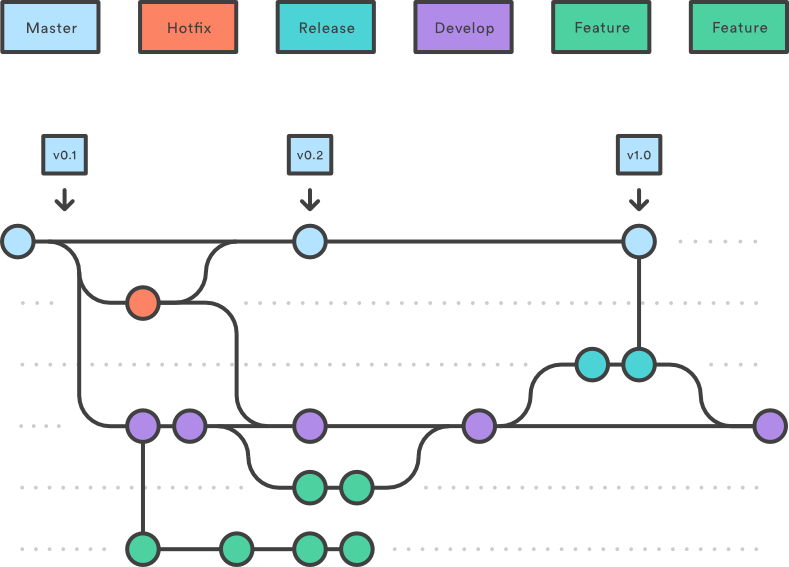
\includegraphics[scale=0.65]{img/gitflow.png}
	\caption{Exemplo de como \emph{GitFlow} funciona, exibindo os diversos \emph{branches} da metodologia.}
\end{figure}

%%%%%%%%%%%%%%%%%%%%%%%%%%%%%%%%%%%%%%%%%%%%%%%%%%%%%%%%%%%%%%%%%%%%%%%%%%%%%%%%%%%%%%%%%
\section{Previsão de Alocação de Recursos}

\subsection*{Recursos Humanos}
\begin{itemize}
	\item 1 Analista de Sistemas S\^enior;
	\item 1 Designer multi-plataforma \emph{freelancer};\footnotemark
	\item 1 Analista de marketing \emph{freelancer} (para o marketing inicial do produto; futuramente, integrar\'a a equipe permanente).
\end{itemize}
\footnotetext{Ou dois designers, sendo um deles webdesigner, e o outro, designer de aplicações móveis}

\subsection*{Recursos Materiais}
\begin{itemize}
	\item Inst\^ancias no \emph{Heroku} (é possível começar com pouco e expandir facilmente no futuro\cite{heroku}) com as seguintes configurações / add-ons:
	\begin{itemize}
		\item \emph{Dynos} (máquinas que processam \emph{requests} web) com \textbf{PHP 5.5}
		\item Servidor \textbf{PostgreSQL}, também facilmente escalável e seguro\cite{heroku-pgsql}
		\item Servidor de \emph{Memcache} \textbf{MemCachier} para caches temporários de aplicação
		\item \textbf{Mandrill by MailChimp} para envio de e-mails de lembretes
		\item \textbf{NewRelic} para monitoria da performance da aplicação e do banco de dados
		\item \textbf{Rollbar} para monitoria de erros nas aplicações
	\end{itemize}
\end{itemize}

%%%%%%%%%%%%%%%%%%%%%%%%%%%%%%%%%%%%%%%%%%%%%%%%%%%%%%%%%%%%%%%%%%%%%%%%%%%%%%%%%%%%%%%%%
\section{Cronograma de Trabalho}
\emph{Diagrama de Gantt.}

%%%%%%%%%%%%%%%%%%%%%%%%%%%%%%%%%%%%%%%%%%%%%%%%%%%%%%%%%%%%%%%%%%%%%%%%%%%%%%%%%%%%%%%%%
\chapter{A Empresa e o Negócio}
\emph{Explicar qual e o objetivo do projeto a curto e medio prazo (objetivos de estudo e de rentabilidade).}

%%%%%%%%%%%%%%%%%%%%%%%%%%%%%%%%%%%%%%%%%%%%%%%%%%%%%%%%%%%%%%%%%%%%%%%%%%%%%%%%%%%%%%%%%
\section{Historico}
\emph{Explicar aqui a experiencia academica e tecnica do criador do sistema (mini-curriculo?)}

%%%%%%%%%%%%%%%%%%%%%%%%%%%%%%%%%%%%%%%%%%%%%%%%%%%%%%%%%%%%%%%%%%%%%%%%%%%%%%%%%%%%%%%%%
\section{Mercado Consumidor}
\emph{Citar alguns grupos de usuarios comuns do sistema}

%%%%%%%%%%%%%%%%%%%%%%%%%%%%%%%%%%%%%%%%%%%%%%%%%%%%%%%%%%%%%%%%%%%%%%%%%%%%%%%%%%%%%%%%%
\section{Concorrencia}
\emph{Falar brevemente sobre as empresas dos produtos concorrentes}

%%%%%%%%%%%%%%%%%%%%%%%%%%%%%%%%%%%%%%%%%%%%%%%%%%%%%%%%%%%%%%%%%%%%%%%%%%%%%%%%%%%%%%%%%
\section{Premissas e Restricoes ao Projeto}
\emph{Explicar as ideias basicas e features essenciais, e o que nao sera possivel fazer no momento ou fica fora do escopo ideal do projeto.}

%%%%%%%%%%%%%%%%%%%%%%%%%%%%%%%%%%%%%%%%%%%%%%%%%%%%%%%%%%%%%%%%%%%%%%%%%%%%%%%%%%%%%%%%%
\chapter{Os Sistemas Atuais}

%%%%%%%%%%%%%%%%%%%%%%%%%%%%%%%%%%%%%%%%%%%%%%%%%%%%%%%%%%%%%%%%%%%%%%%%%%%%%%%%%%%%%%%%%
\section{Principais Concorrentes}
\emph{Descrever os principais sistemas do mercado atual, como Granatum, Mint, Monefy, Yupee, etc}

%%%%%%%%%%%%%%%%%%%%%%%%%%%%%%%%%%%%%%%%%%%%%%%%%%%%%%%%%%%%%%%%%%%%%%%%%%%%%%%%%%%%%%%%%
\section{Outros Sistemas}
\emph{Explicar sobre outras formas de organizacao financeira e suas vantagens e desvantagens, como o uso de um caderno manual, ou planilhas eletronicas.}

%%%%%%%%%%%%%%%%%%%%%%%%%%%%%%%%%%%%%%%%%%%%%%%%%%%%%%%%%%%%%%%%%%%%%%%%%%%%%%%%%%%%%%%%%
\section{Motivacao para o Novo Sistema}
\emph{Porque o nosso sistema seria melhor que os atuais?}

%%%%%%%%%%%%%%%%%%%%%%%%%%%%%%%%%%%%%%%%%%%%%%%%%%%%%%%%%%%%%%%%%%%%%%%%%%%%%%%%%%%%%%%%%
\subsection{Problemas dos Sistemas Atuais}
\emph{Desvantagens da concorrencia}

%%%%%%%%%%%%%%%%%%%%%%%%%%%%%%%%%%%%%%%%%%%%%%%%%%%%%%%%%%%%%%%%%%%%%%%%%%%%%%%%%%%%%%%%%
\subsection{Situacao Desejada}
\emph{Objetivos do nosso sistema}

%%%%%%%%%%%%%%%%%%%%%%%%%%%%%%%%%%%%%%%%%%%%%%%%%%%%%%%%%%%%%%%%%%%%%%%%%%%%%%%%%%%%%%%%%
\chapter{O Sistema Proposto}

%%%%%%%%%%%%%%%%%%%%%%%%%%%%%%%%%%%%%%%%%%%%%%%%%%%%%%%%%%%%%%%%%%%%%%%%%%%%%%%%%%%%%%%%%
\section{Requisitos do Sistema}

%%%%%%%%%%%%%%%%%%%%%%%%%%%%%%%%%%%%%%%%%%%%%%%%%%%%%%%%%%%%%%%%%%%%%%%%%%%%%%%%%%%%%%%%%
\section{Casos de Uso}

%%%%%%%%%%%%%%%%%%%%%%%%%%%%%%%%%%%%%%%%%%%%%%%%%%%%%%%%%%%%%%%%%%%%%%%%%%%%%%%%%%%%%%%%%
\subsection{Diagramas}

%%%%%%%%%%%%%%%%%%%%%%%%%%%%%%%%%%%%%%%%%%%%%%%%%%%%%%%%%%%%%%%%%%%%%%%%%%%%%%%%%%%%%%%%%
\subsection{Especificacoes}

%%%%%%%%%%%%%%%%%%%%%%%%%%%%%%%%%%%%%%%%%%%%%%%%%%%%%%%%%%%%%%%%%%%%%%%%%%%%%%%%%%%%%%%%%
\section{Diagrama Geral de Fluxo de Comunicacao (Topologia?)}
\emph{Indicar aqui o fluxo de comunicacao entre o servidor REST e os mecanismos de cache da rede e dos aplicativos web e mobile.}

%%%%%%%%%%%%%%%%%%%%%%%%%%%%%%%%%%%%%%%%%%%%%%%%%%%%%%%%%%%%%%%%%%%%%%%%%%%%%%%%%%%%%%%%%
\section{Modelo Conceitual de Classes / Servicos REST}
\emph{Provavelmente muito similar ao modelo de dados, visto que os objetos do servidor REST serao todos modelos de dados, e a principio nao faz sentido fazer modelagem de classes de sistemas JS (que sao orientados a prototipos e nao tem heranca nativamente). Portanto, talvez seja substituido por uma previa dos servicos REST que poderiam ser fornecidos.}

%%%%%%%%%%%%%%%%%%%%%%%%%%%%%%%%%%%%%%%%%%%%%%%%%%%%%%%%%%%%%%%%%%%%%%%%%%%%%%%%%%%%%%%%%
\section{Modelo Conceitual de Dados}
\emph{Auto-explicativo.}

%%%%%%%%%%%%%%%%%%%%%%%%%%%%%%%%%%%%%%%%%%%%%%%%%%%%%%%%%%%%%%%%%%%%%%%%%%%%%%%%%%%%%%%%%
\printbibliography

\end{document}